\chapter{Medical Background}
In this chapter, a short description of the problem setting from a medical point of view is given. If not specified, the information given below is based on the textbook "Human Anatomy and Physiology", by Van Wynsberghe, Noback, and Carola \cite{VanW95}
\section{Anatomy of the central nervous system}
The human nervous system consists of peripheral nervous system, and the central nervous system (CNS). The former consists of spinal and cranial nerves and sensory receptor organs while the latter constits of two parts: the brain and the spinal cord. The CNS receives and process information from all parts of the body. Consequently, studies on the CNS are crucial for our understanding of the human anatomy.
\section{The Spinal Cord}
\begin{center}
\begin{figure}[!ht]
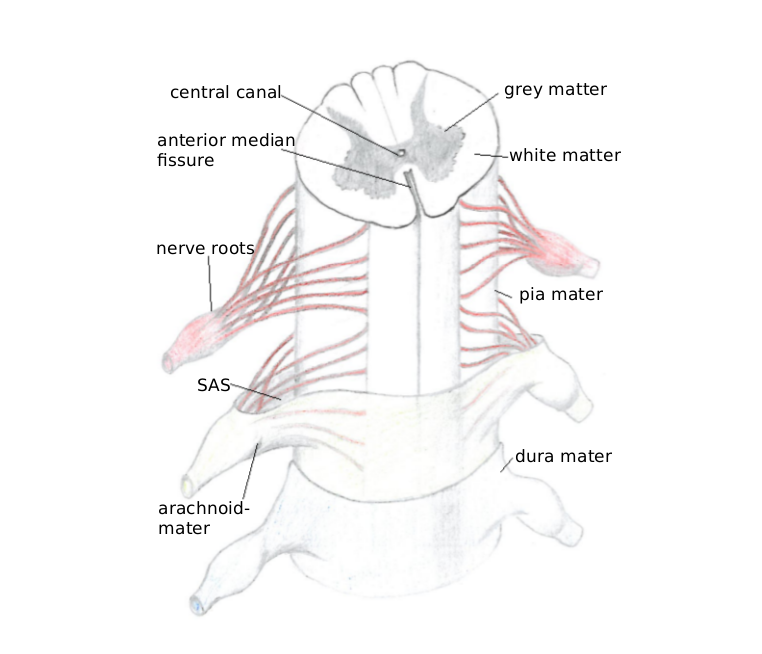
\includegraphics[scale=0.3]{figures/Spinal_Cord} \\
\caption{Schematic figure of the spinal cord. The pia mater surrounds the spinal cord, and between the pia mater and dura mather lies the subarachnoid space where CSF flows} \label{fig:Cord}
\end{figure}
\end{center}
The spinal cord carries information between the body and the brain and is divided into four or five regions from top to bottom: Cervical (C), thoracic (T), lumbar (L) and sacral (S) in addition to the coccygeal part at the very bottom. The upper end of the spinal cord is continuous with the lowermost part of the brain, while the lower part tapers at the filum terminale, which attatches to the coccyx, known as the tailbone. Along the cord, there are 31 pairs of nerves exiting the cord: 8 in the cervical region, 12 in the thoracic region, 5 in the lumbar region, 5 in the sacral region and one in the coccygeal region. The first four segments of the cord are given names C1-C8, T1-T12, L1-L5, S1-S5. The tissue within the spinal cord consists of nervous tissue in form of white and grey matter which differs in both structure and function. In the center of the spinal cord, lies a tiny central spinal canal where CSF can flow. This channel closes off with age. Surrounding the central canal lies the gray matter in an H-shape, similar to a butterfly. The rest consists of white matter, and the ratio between white and gray matter differs along the spinal cord. 
\\
\\
There are three layers covering the brain and spinal cord known as meninges. The innermost layer surrounds the spinal cord and is known as the \textit{pia mater}. The pia contains blood vessels that nourish the spinal cord. The middle layer, the \textit{arachnoid} runs caudally extending almost all the way down the spinal cord. At the S2 vertebral level, the arachnoid joins the filum terminale. The outermost layer of the meninges protecting the spinal cord is known as the \textit{dura mater} and is a though fibrous membrane. 
\\
\section{The Chiari malformation}
The Chiari malformation, also known as Arnold-Chiari Malformation is a neurological condition where a displacement of the cerebellum, or more presice the cerebellar tonsils, down through the foramen magnum occour. The condition is classified into four stages I-IV where IV is the most severe. In a Chiari patient, the cerebellar tonsils obstructs the CSF flow (see figure \ref{fig:CSF}) and even Chiari I patients have shown to have greater CSF velocities and a more complex flow pattern than healty subjects. \cite{Quig04} These patients could also experience severe headache, dizziness, tinnitus and muscle weakness. As the cerebellum is part of the brain that controls balance, loss of coordination have also been reported. 
\begin{figure}[!ht]
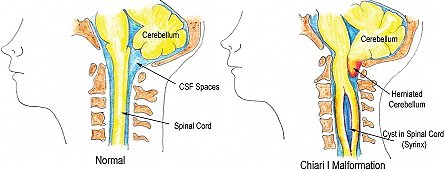
\includegraphics[scale=0.8]{figures/Ida_CSF.png} \\
\caption{The Chiari malformation. Healthy subject to the left and a downward displacement of the cerebellar tonsils on the right} \label{fig:CSF}
\end{figure}
\subsection{Syringomelia}
In some cases, Chiari patients develops a fluid cavity, known as a syrinx within the spinal cord. Some of the symptoms are similar to the Chiari patients in general, but include muscle and back pain, weakness, numbness and iniabilities to feel temperature changes. Many theories on the pathogenesis of syringomelia have been proposed, but the details are not yet fully understood. In patients diagnosed with Chiari I, about 2/3 develops syrinxes within the spinal cord tissue. Thus, not all Chiari patients have syringomelia and in addition patients with syringomeila does not necessary have the Chiari malformation. Thompson et al. have in a recent study suggested the anatomy of the cervical (upper part) spinal canal plays a role in the formation of syrnixes. \cite{Thom15} The study showed that Chiari patients with syringomelia had greater \textit{C4-C7}-tapering of the cervical spinal canal, but no significant difference on \textit{C1-C4}-tapering. Tapering is the narrowing of the spinal canal in the downwards, or caudal direction. 
\\
\\
Most researchers seem to agree on the fact that altered CSF dynamics is associated with the formation of the syrinx. 
